\def\widerface{
    Bộ dữ liệu WIDER FACE \cite{yang2016wider} là một bộ dữ liệu nổi tiếng được sử dụng rộng rãi dành cho bài toán face detection.
    Bộ dữ liệu WIDER FACE được nhóm tác giả nhấn mạnh về tính thực tiễn do có chứa ảnh đa dạng và gần với các khung cảnh trong thực tế.
    Bộ dữ liệu chứa rất nhiều ảnh với các khuôn mặt đa dạng trong tỷ lệ kích thước, kiểu dáng, biểu cảm, che chắn, góc quay và ánh sáng.
    Hơn nữa số lượng ảnh của bộ WIDER FACE cũng lớn hơn rất nhiều so với các bộ dữ liệu về mặt ở thời điểm đó.

    \begin{figure}[H]
        \centering
        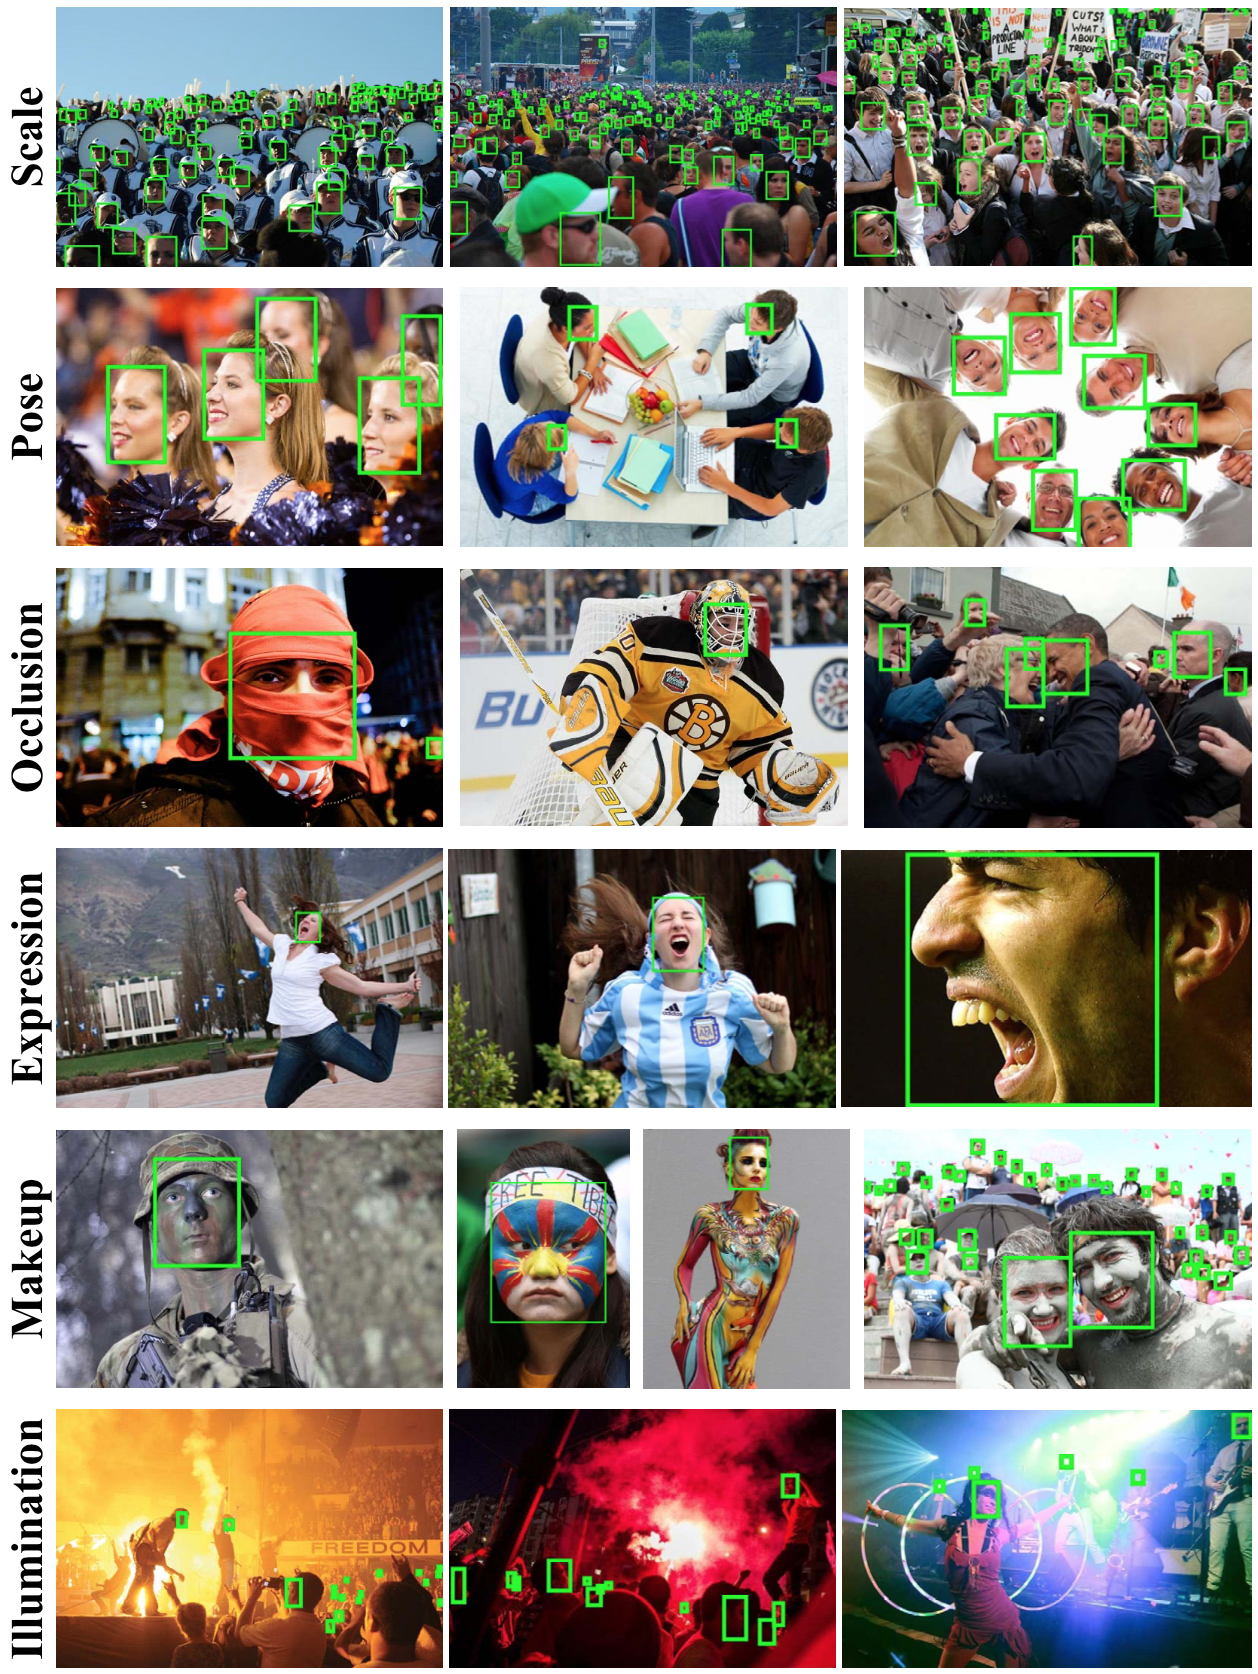
\includegraphics[width=15cm] {images/widerface_examples}
        \caption{Một số ví dụ trong bộ dữ liệu WIDER FACE (Nguồn: \cite{yang2016wider})}
        \label{fig:widerface_examples}
    \end{figure}

    \noindent
    \textbf{\textit{Các thông số của bộ dữ liệu WIDER FACE}} \\
    Bộ dữ liệu WIDER FACE bao gồm 32,203 ảnh với 393,703 bbox của khuôn mặt với sự đa dạng về kích thước, góc quay, che chắn.
    Bộ dữ liệu WIDER FACE được chụp từ 61 khung cảnh khác nhau, trong đó, với mỗi khung cảnh, nhóm tác giả chia thành ba bộ train/val/test theo tỷ lệ 40\%/10\%/50\%.

    \begin{figure}[H]
        \centering
        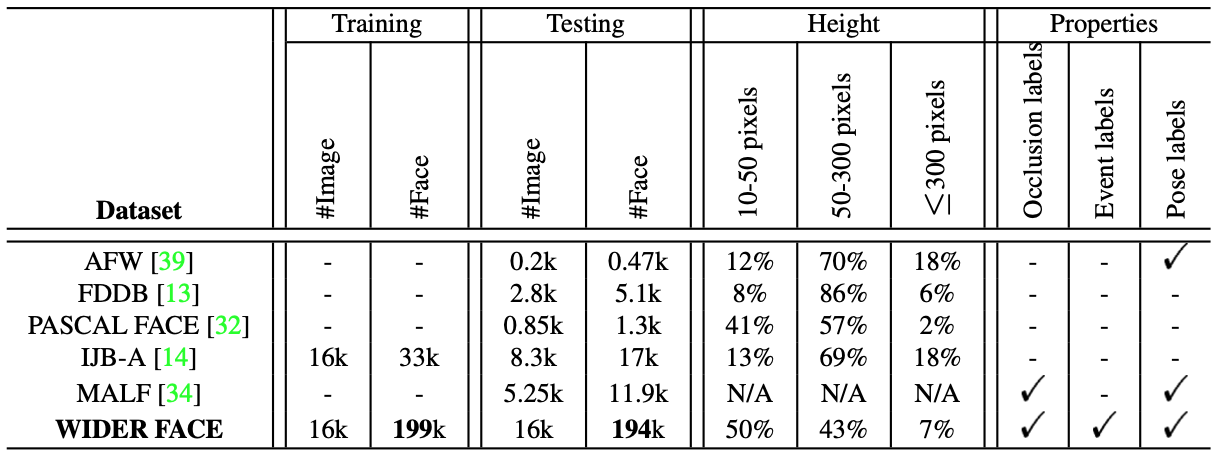
\includegraphics[width=15cm] {images/widerface_compare_1}
        \caption{So sánh về số lượng và độ đa dạng của bộ dữ liệu WIDER FACE với một số bộ dữ liệu khác (Nguồn: \cite{yang2016wider})}
        \label{fig:widerface_compare_1}
    \end{figure}
    
    \noindent
    Nhóm tác giả của bộ dữ liệu WIDER FACE sử dụng mô hình EdgeBox \cite{zitnick2014edge} để chia bộ dữ liệu thành ba mức độ khó (bộ Dễ, bộ Trung bình và bộ Khó).
    Trong đó, mô hình EdgeBox đạt mức recall lần lượt tương ứng với bộ Dễ, bộ Trung bình và bộ Khó là 92\%, 76\% và 34\%.
    Mô hình EdgeBox đạt kết quả kém hơn rất nhiều trên bộ WIDER FACE so sánh với kết quả trên các bộ dữ liệu khác.

    \begin{figure}[H]
        \centering
        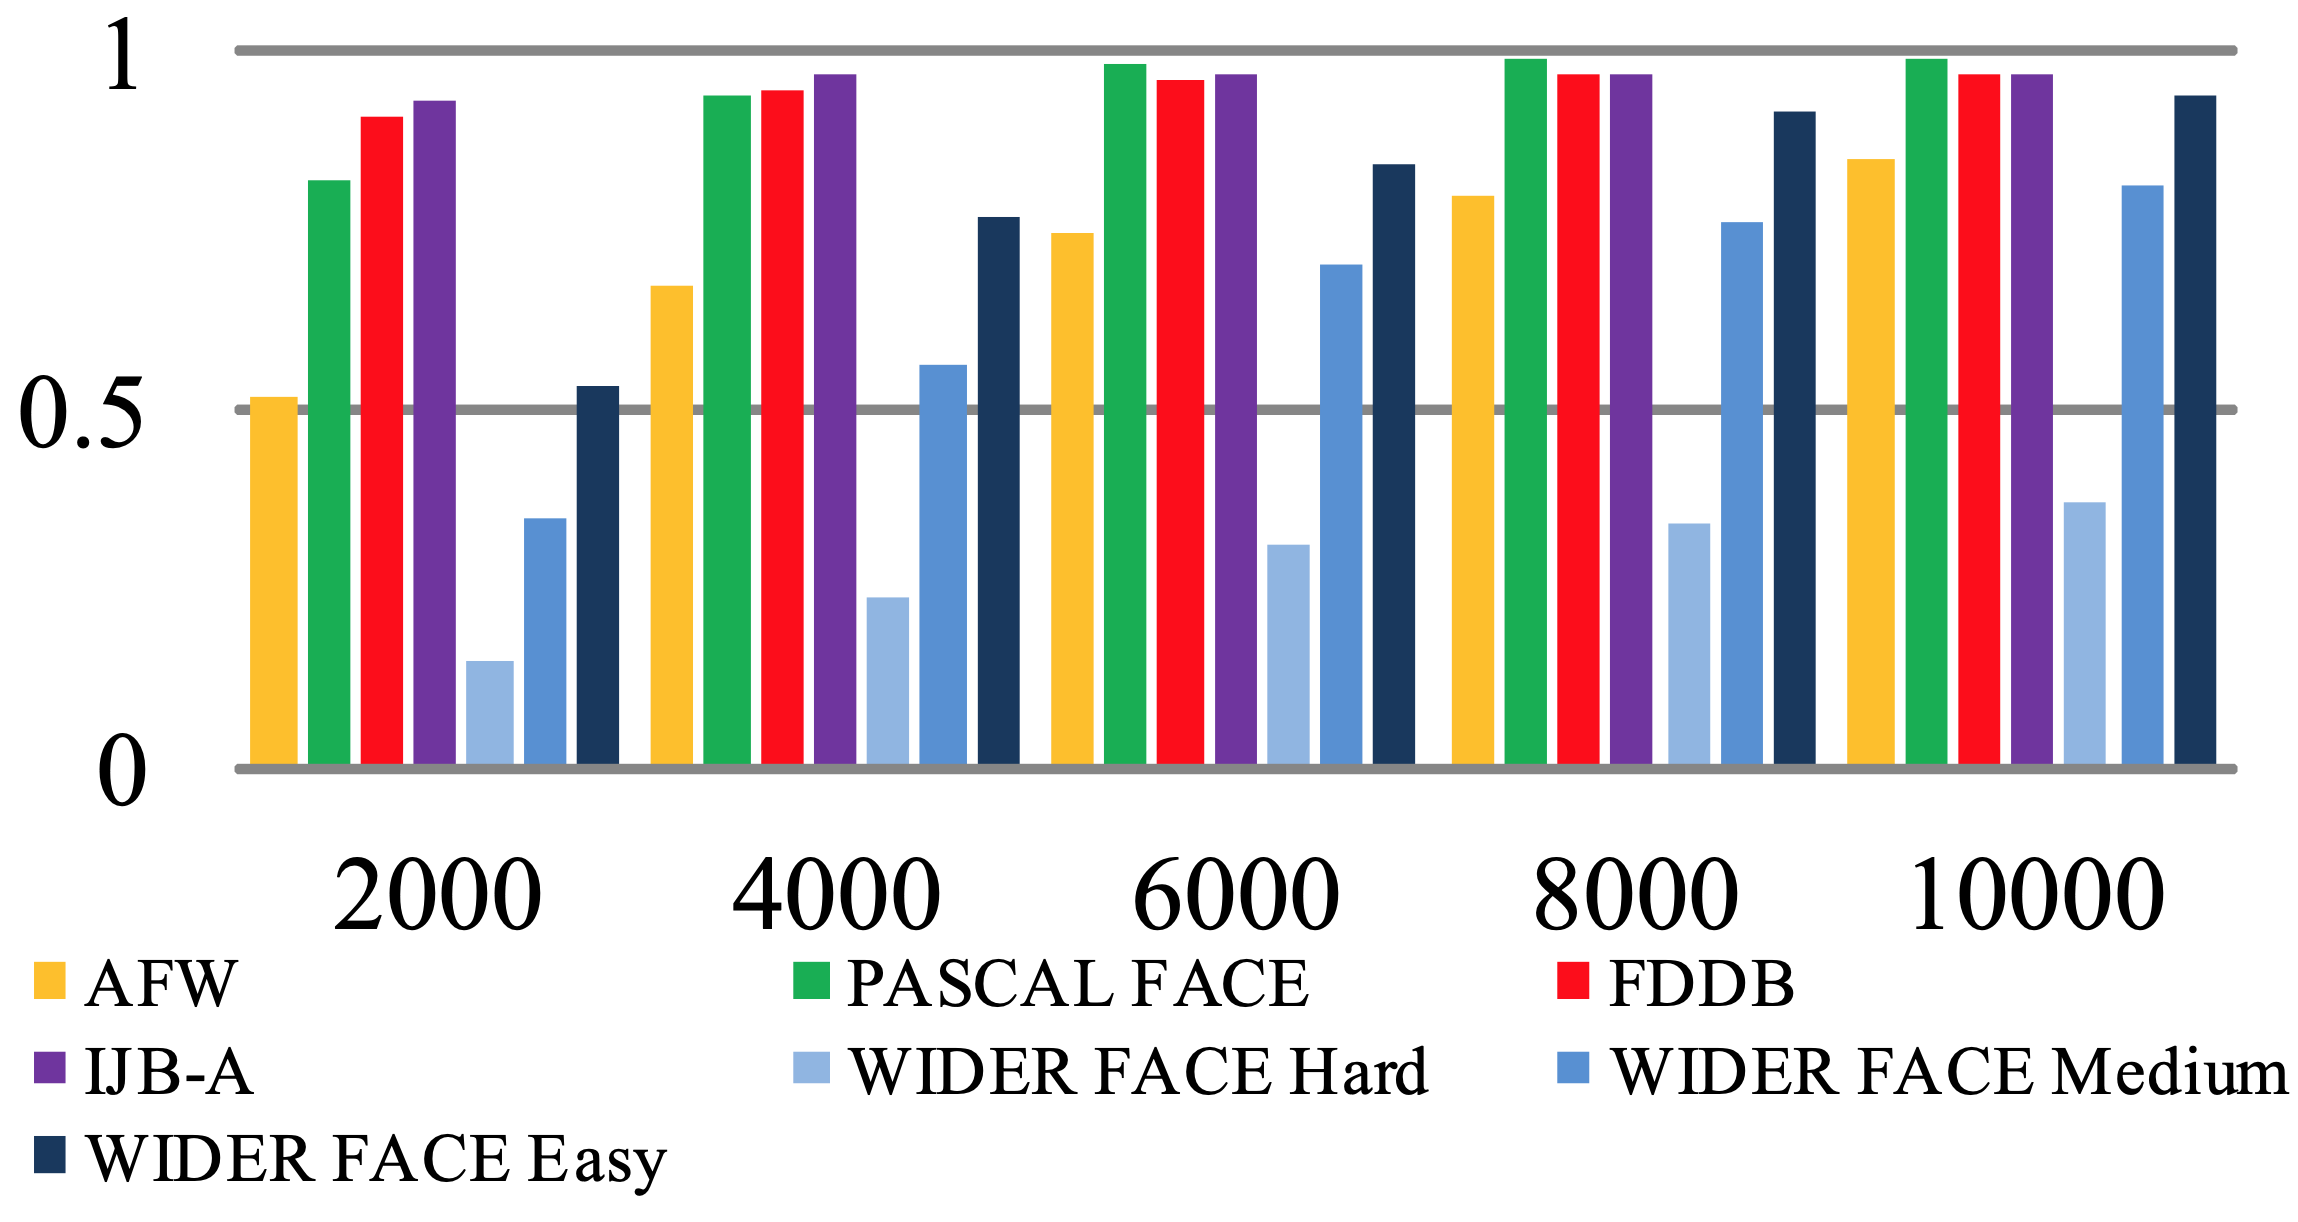
\includegraphics[width=15cm] {images/widerface_compare_2}
        \caption{So sánh độ khó của bộ dữ liệu WIDER FACE với một số bộ dữ liệu khác (Nguồn: \cite{yang2016wider})}
        \label{fig:widerface_compare_2}
    \end{figure}

    \noindent
    \textbf{\textit{Bộ dữ liệu WIDER FACE với landmarks}} \\
    Nhóm tác giả của mô hình RetinaFace \cite{deng2020retinaface} đã bổ sung thêm vào bộ dữ liệu WIDER FACE thông tin về landmarks của các khuôn mặt bao gồm 5 điểm: tâm của mắt trái, tâm của mắt phải, đỉnh của mũi, điểm mép miệng trái và điểm mép miệng phải.

    \begin{figure}[H]
        \centering
        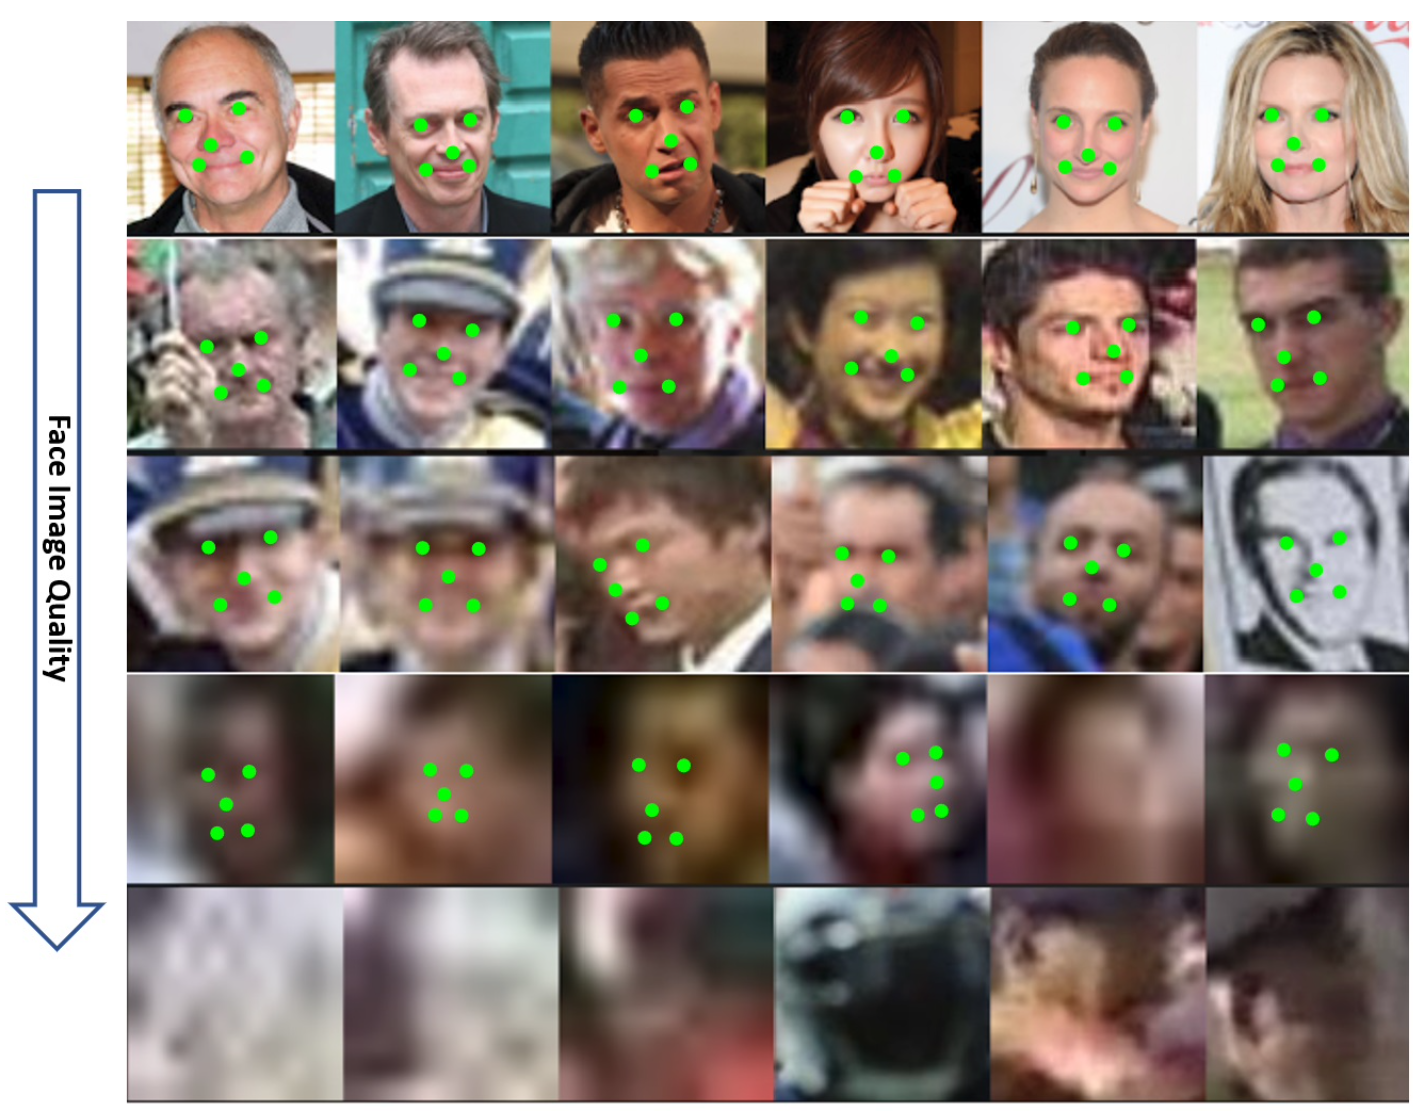
\includegraphics[width=10cm] {images/widerface_five_levels_lm_1}
        \caption{Ví dụ về năm mức độ khó của khuôn mặt trong việc gán landmarks (Nguồn: \cite{deng2020retinaface})}
        \label{fig:widerface_five_levels_lm_1}
    \end{figure}

    \noindent
    Dựa vào chất lượng của ảnh, nhóm tác giả đã chia bộ dữ liệu thành 5 mức độ khó: \\
    - Độ khó 1 (dễ nhất): Dễ dàng gán nhãn được 68 điểm landmarks của mặt. \\
    - Độ khó 2: Có thể gán nhãn được 68 điểm landmarks của mặt. \\
    - Độ khó 3: Dễ dàng gán nhãn được 5 điểm landmarks của mặt. \\
    - Độ khó 4: Có thể gán nhãn được 5 điểm landmarks của mặt. \\
    - Độ khó 5 (khó nhất): Chỉ có thể phân biệt được với background của ảnh. Với các bounding box ở mức độ khó này, nhóm tác giả không gán 5 điểm landmarks. \\
    Dựa vào các mức độ khó nói trên, nhóm tác giả của RetinaFace đã gán landmarks cho các khuôn mặt trong hai tập dữ liệu train và val, tương ứng 84.6k mặt cho tập train và 18.5k mặt cho bộ val.

    \begin{figure}[H]
        \centering
        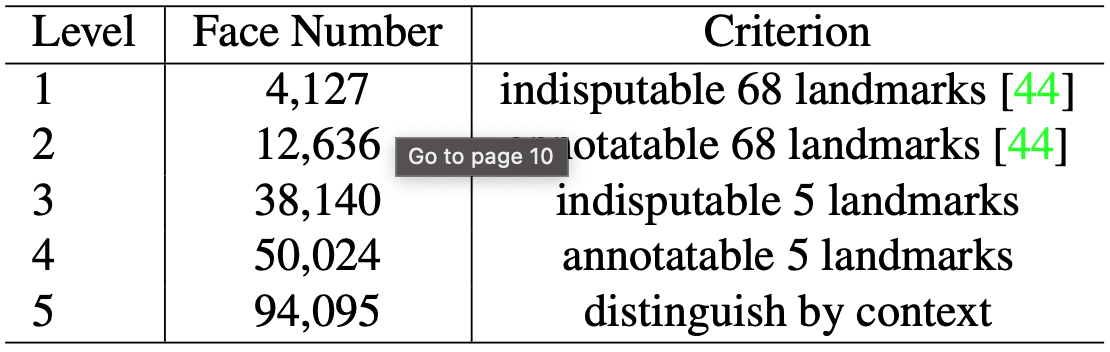
\includegraphics[width=10cm] {images/widerface_five_levels_lm_2}
        \caption{Các thông số của năm mức độ khó của khuôn mặt trong việc gán landmarks (Nguồn: \cite{deng2020retinaface})}
        \label{fig:widerface_five_levels_lm_2}
    \end{figure}

    \noindent
    \textbf{\textit{Vấn đề tồn đọng của bộ dữ liệu WIDER FACE}} \\
    Ở thời điểm ra mắt, bộ dữ liệu WIDER FACE thật sự là một bước tiến về dữ liệu cho bài toán face detection bởi số lượng và sự đa dạng.
    Tuy nhiên, cho đến nay, kích thước như ảnh trong bộ WIDER FACE khoảng 1000 - 1500 pixel không còn là kích thước lớn nữa.
    Điều này là rào cản cho giới nghiên cứu khi phát triển các mô hình giải quyết bài toán face detection trong ảnh chất lượng cao.
}